\documentclass{article} 
\usepackage[utf8]{s} 

\usepackage{listings} 
\usepackage{xcolor} 
\usepackage{graphicx} 
\usepackage{caption} 
\usepackage{subcaption} 
\usepackage{float}  
\usepackage{wrapfig} 
\graphicspath{ {./Image/} } 

\definecolor{codegreen}{rgb}{0,0.6,0} 
\definecolor{codegray}{rgb}{0.5,0.5,0.5} 
\definecolor{codepurple}{rgb}{0.58,0,0.82} 
\definecolor{backcolour}{rgb}{0.95,0.95,0.92} 

\lstdefinestyle{mystyle}{ 
    backgroundcolor=\color{backcolour},    
    commentstyle=\color{codegreen}, 
    keywordstyle=\color{magenta}, 
    numberstyle=\tiny\color{codegray}, 
    stringstyle=\color{codepurple}, 
    basicstyle=\ttfamily\footnotesize, 
    breakatwhitespace=false,          
    breaklines=true,                  
    captionpos=b,                     
    keepspaces=true,                  
    numbers=left,                     
    numbersep=5pt,                   
    showspaces=false,                 
    showstringspaces=false, 
    showtabs=false,                   
    tabsize=4 
} 

\title{Mini Project 1: Filtering and image restoration} 
\author{Jeppe Matzen} 
\date{September 2020} 

\begin{document} 
\lstset{style=mystyle} 
\maketitle 

\section{Aim:} 

Målet med mini projekt 1 er at overfører teori til $C++$ kode ved at implementere funktioner og anvende funktionerne på virkelige medicinske billeder. \newline 
For selv at kunne konstruere $C++$ funktioner fra bunden er det nødvendigt at forstå formålet og fremgangsmåden detaljeret.   

  

\section{Method:} 
\subsection{Opgave 2} 

Opgaven to bad om at få udregnet og tegnet et gray-level-histogram over gray-values. \newline 
Det gråtoner billede der arbejdes med i denne opgave, er et $2^8$ bits bilede, bestående af pixel værdier fra 0-255. 0 svarer til sort og 255 til hvid. \newline 
For at kunne udregne histogrammet tælles frekvensen af hver pixel. Frekvensen normaliseres herefter ved at dividere med det totale antal pixel (Rækker * Kolonner). Dette giver et "probability density function" (PDF), som indeholder sandsynligheden fra 0-1 for at observere en bestemt pixel. Det normaliserede histogram er et godt værktøj til at danne et overblik over fordelingen af pixel i et billede. \newline 

\subsection{Opgave 3} 

I opgave tre skulle der laves et stretch på histogrammet fra opgave to. Dette gøres for at udnytte hele den dynamiske pixel range. Et stretch udvider range fra at gå fra billedets min til max til at gå fra, i det her tilfælde 0 til 255. Dette ændrer ikke i udformningen af histogrammet, men flader det ud. Til dette benyttes formlen $$g_i = \frac{2^n - 1}{a_{max} - a_{min}} * a_i $$ \newline Hvor n er antallet af bits, $a_{max}$ er den største pixel værdi og $a_{min}$ er den mindste pixel værdi. 
Histogram stretch bruges til at øge kontrasten af et billede, der er forskellen mellem den højeste og den mindste pixel. Ofte vil der sættes en grænseværdi for at undgå at outlier i billedet har indflydelse på hvor meget histogrammet kan strækkes. 

  

\subsection{Opgave 4}, 

I opgave fire skulle billedet inverteres. I dette tilfælde var det et billede med pixels i rækkevidden 0-255. For at invertere billedet blev der udregnet en ny værdi for hver pixel i billedet med formlen $$ invertedPixelValue = 255 - oldPixelValue $$ \newline 
Ved at invertere billedet bliver de lyse pixels mørke og omvendt. Dette kan gøre det muligt at fremhæve ting i billedet.   

\subsection{Opgave 5} 

I opgave fem skulle der køres et tre gange tre filter på billedet. For at benytte et filter er det nødvendt at "padde" eller tilføje en ramme rundt om billedet. Padding kan enten være lavet med nuller eller gennemsnitsværdien af de nærmeste naboer. Det gøres for at billedet ikke bliver mindre hver gang filteret bruges på billedet. \newline 
Et tre gange tre gennemsnits filter, som er brugt i denne opgave, fungere ved at det stiller sig på en pixel, og regner summen af de otte pixels, der ligger omkring og den selv, hvorefter der divideres med størrelsen af filteret. På denne måde bliver hver pixel udskiftet med gennemsnittet af den selv og de omkring liggende.  
Dette bruges ofte til at udglatte et billede for at fjerne støj. Det vil få billedet til at se mere "grumset" ud. 

  

\subsection{Opgave 6} 

I opgave seks skulle størrelsen på filteret ændre til et fem gange fem filter og efterfølgende skulle det ændres fra et gennemsnits filter til et gausian filter. \newline 
Ved at øge filter størrelsen mindsker man sensitivitet over før støj men på bekostning af at man udglatter skarpe overgange som f.eks. kanter i billedet. \newline 
Gausian filteret er forskellige fra gennemsnits filteret ved at hver pixel er vægtet efter en gausian fordeling i stedet for at alle har vægten 1. Den højst vægtet pixel er den midterste og dets længere man kommer fra centrum dets lavere vægtet er pixelen.\newline 
Gausian filteret og gennemsnits filteret bruges begge at fjerne støj.\newline 

\section{Results:  describe the outcome of applying the tools on the images and reflect on how these tools could be used to improve the usage of the images} 

  

Billedet der bliver arbejdet med i opgave to til opgave seks er dette billede af en lunge \ref{fig:image1} \ref{fig:f1}.\newline 

  

\subsection{Opgave 2} 

Histogrammet viser fordelingen af pixels i billedet. Det ses at største delen af pixels ligger i den venstre del af histogrammet hvilket betyder at det hovedsageligt består af lyse gråtoner. Ud fra histogrammet kan det vurderes om det ville give mening af strække billedet og hvilken thredshold værdi der ville være god for billedet. Forholdet i histogrammet er skaleret til vindue størrelsen. 

  

\begin{figure}[!h] 
  \begin{subfigure}[b]{0.49\linewidth} 
    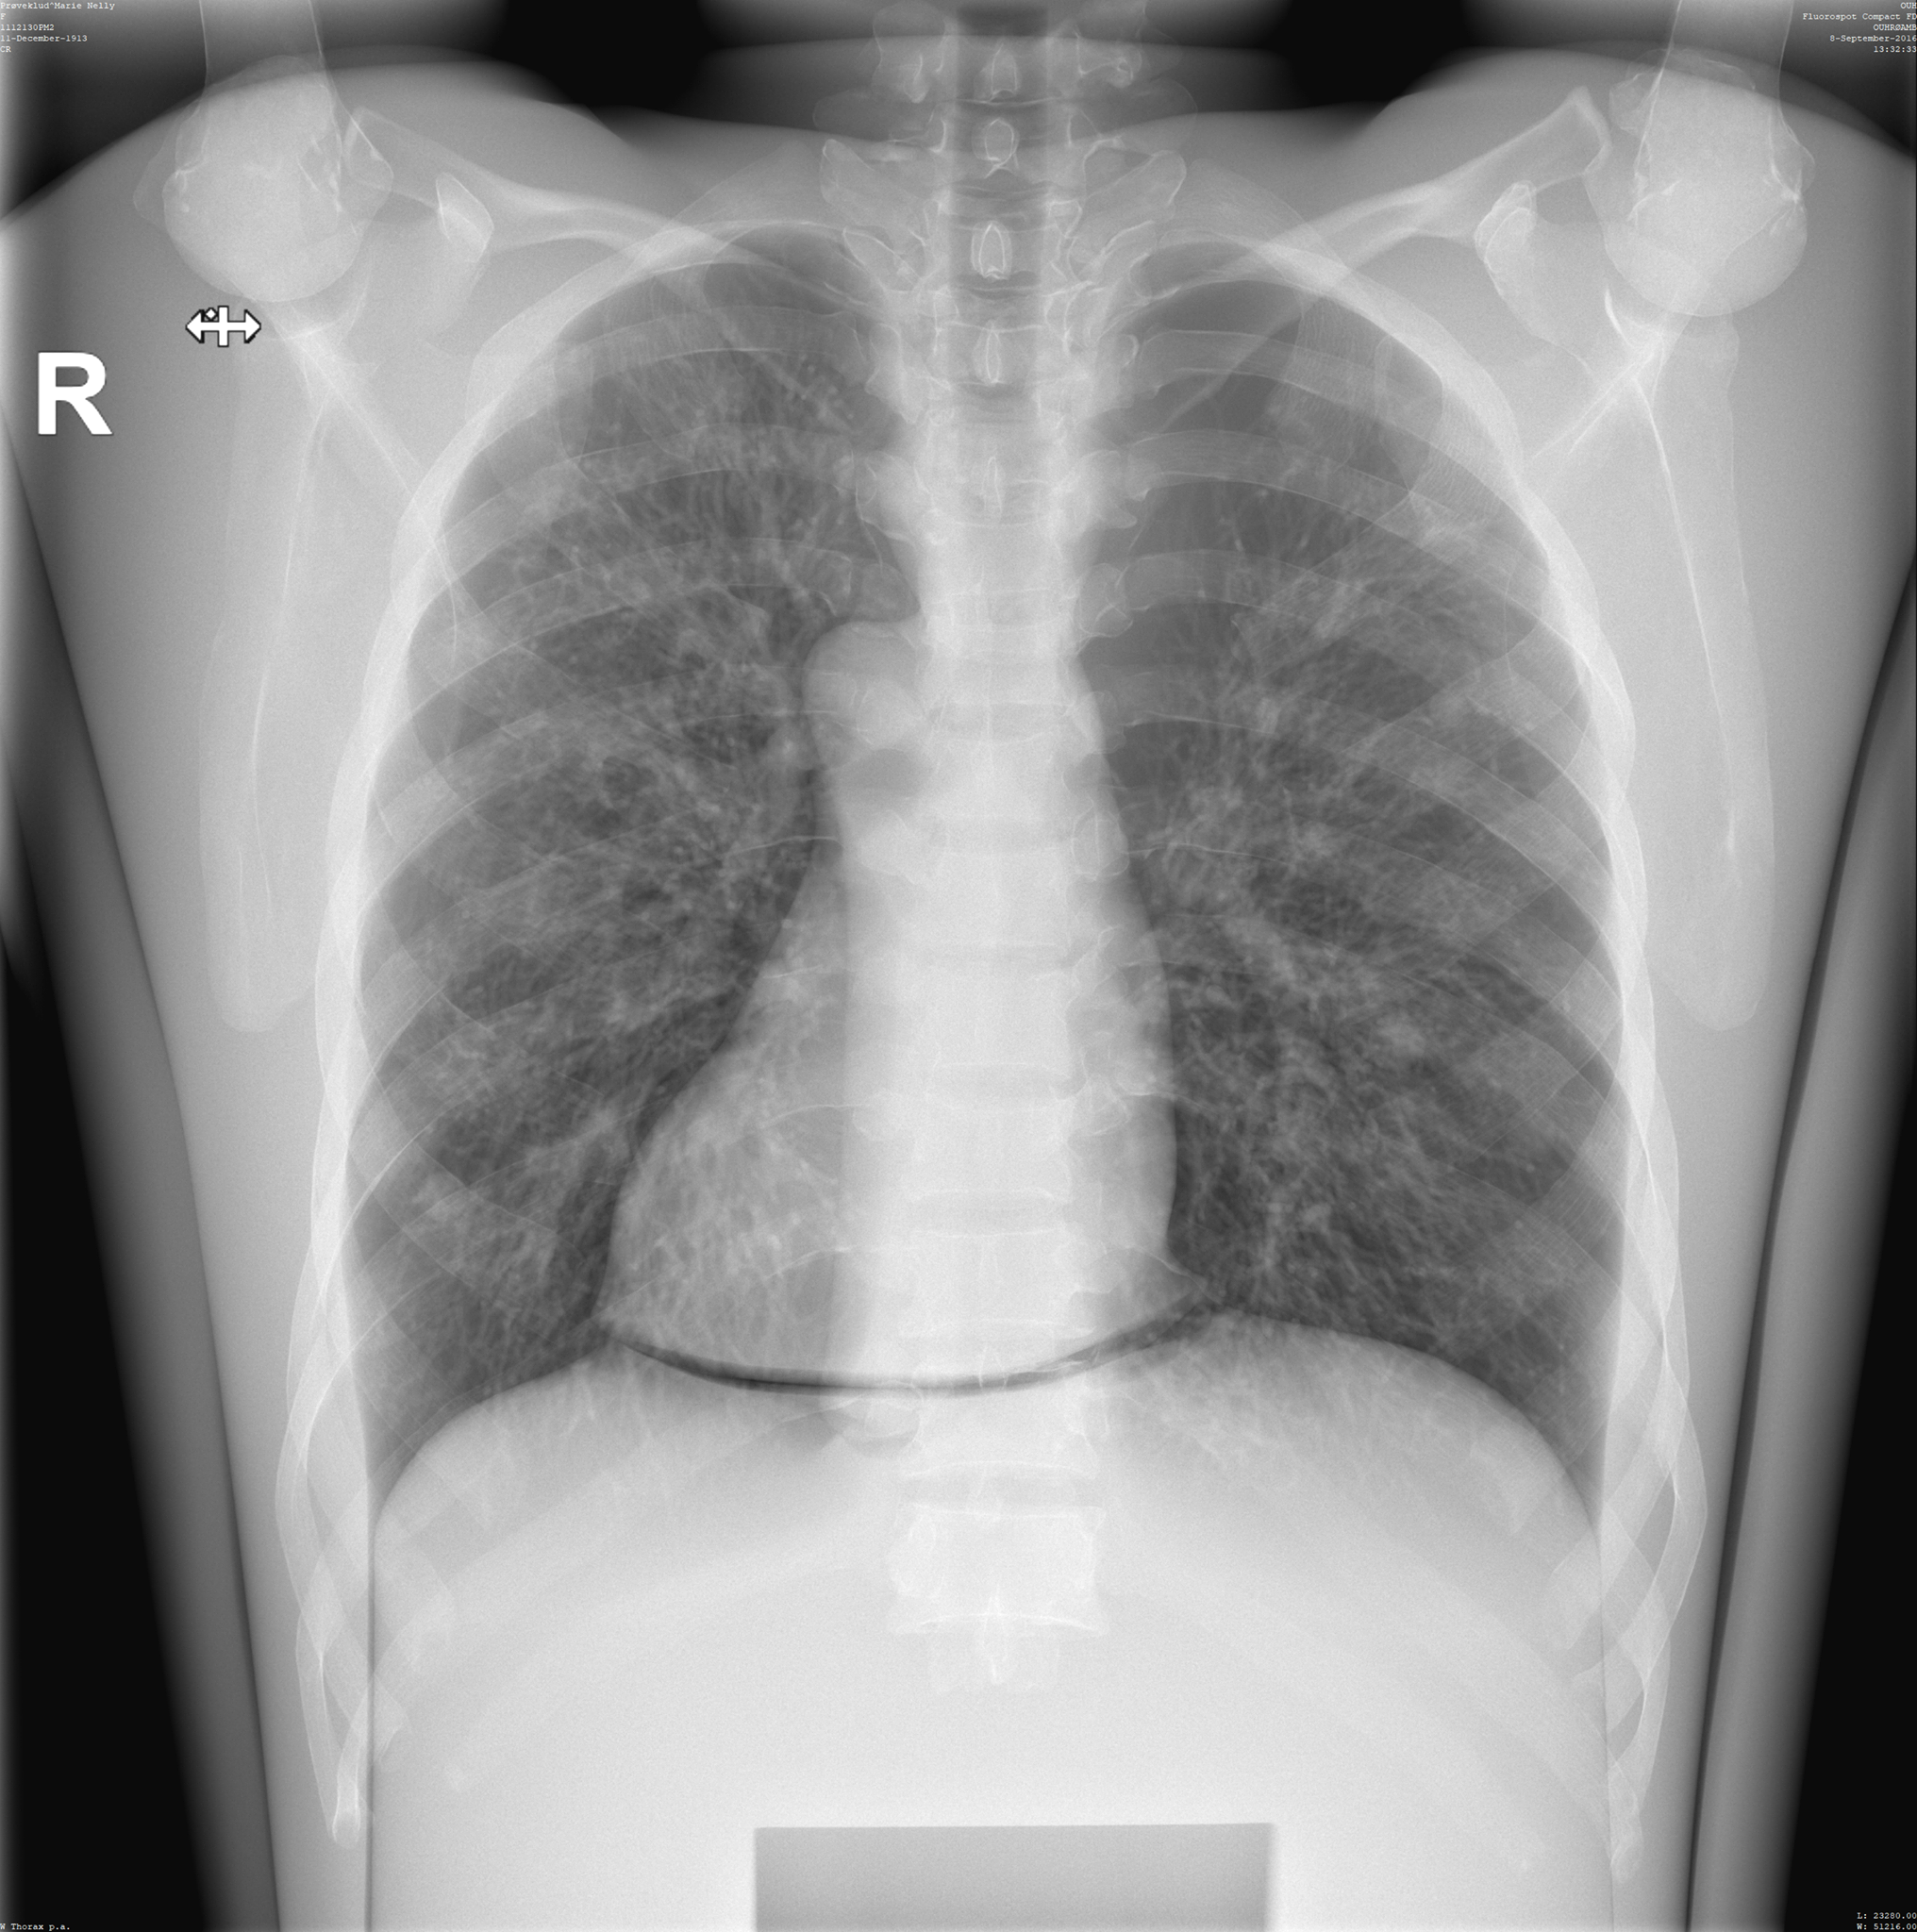
\includegraphics[width=\linewidth]{Image/lung.png} 
    \caption{Billede af lunge.} 
    \label{fig:f1} 
  \end{subfigure} 
  \hfill 
  \begin{subfigure}[b]{0.49\linewidth} 
    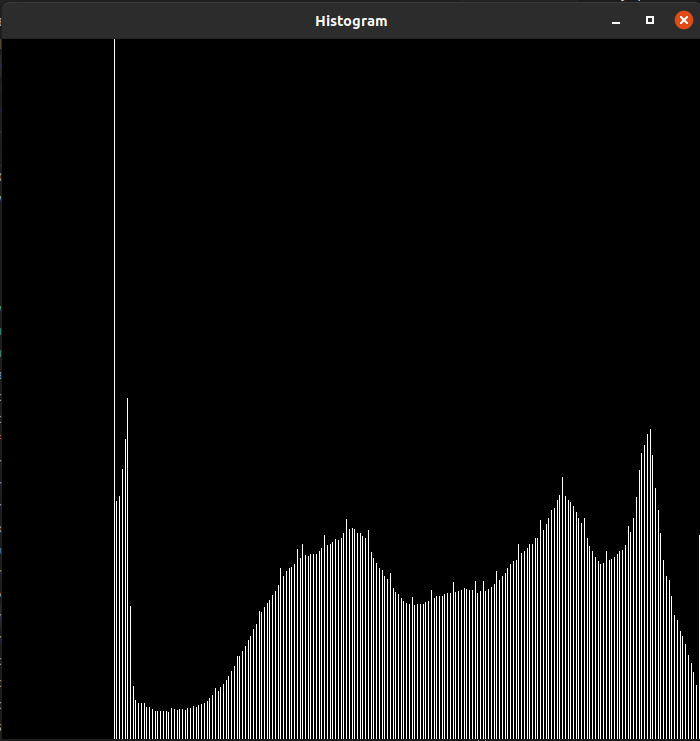
\includegraphics[width=\linewidth]{Image/Histogram.png} 
    \caption{Histogram af lunge billede} 
    \label{fig:f2} 
  \end{subfigure} 
      \caption{} 
    \label{fig:image1} 
\end{figure} 

  

\subsection{Opgave 3} 

Efter histogrammet er blevet strækket, er Det første Spike rykket helt til venstre og histogrammet er blevet fladere. Dette resulterer i at hele den dynamiske range er blevet udnyttet. Det giver et mere tydeligt billede fordi der er stører forskel i kontrasten.  

\begin{figure}[H] 
     \begin{center} 
        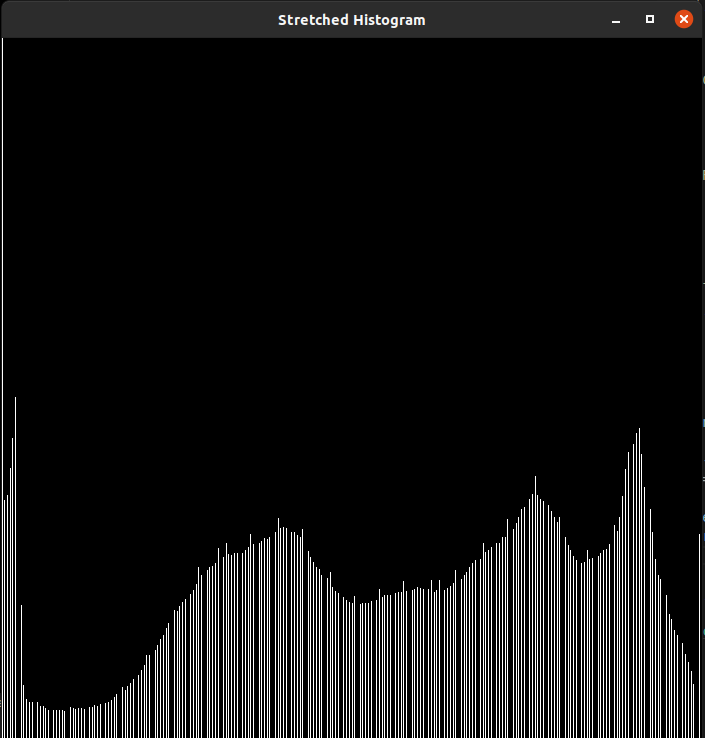
\includegraphics[width=0.5\textwidth]{Image/StrechedHistogram.png} 
        \caption{Stretched histogram af lunge billede} 
    \end{center} 
    \label{fig:f3} 
\end{figure} 

\subsection{Opgave 4} 

På figur \ref{fig:f4} ses det inverterede billede af en lunge. Dette fremhæver nogen farve forskelle som ellers ikke var så tydelige i det originale billede.  

\begin{figure}[H]  
  \begin{center} 
    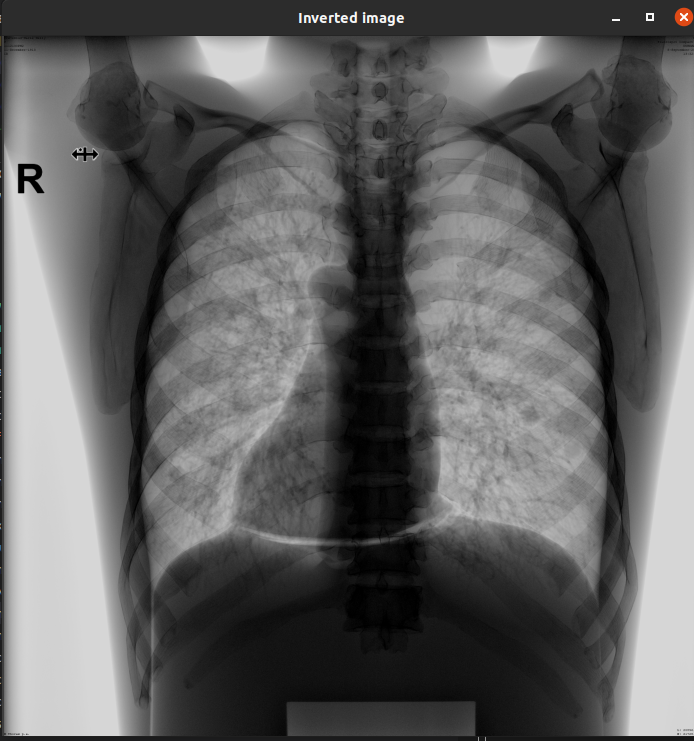
\includegraphics[width=0.48\textwidth]{Image/InvertedImage.png} 
  \end{center} 
  \caption{Inverterede af lunge billede} 
  \label{fig:f4} 
\end{figure} 

\subsection{Opgave 5} 

På figur \ref{fig:image2} ses på billede (a) det originale billede af en lunge og på billede (b) lugen med et 3X3 filter. På det filtrerede billede ses en større forskel i farve. Dette skaber et mere tydeligt billede og gør det nemmere at identificere strukturer i billedet.\newline 
Ulempen er at kanter bliver mere udtværet, men med et 3X3 filter er dette minimalt.  

\begin{figure}[H] 
  \begin{subfigure}[b]{0.49\textwidth} 
    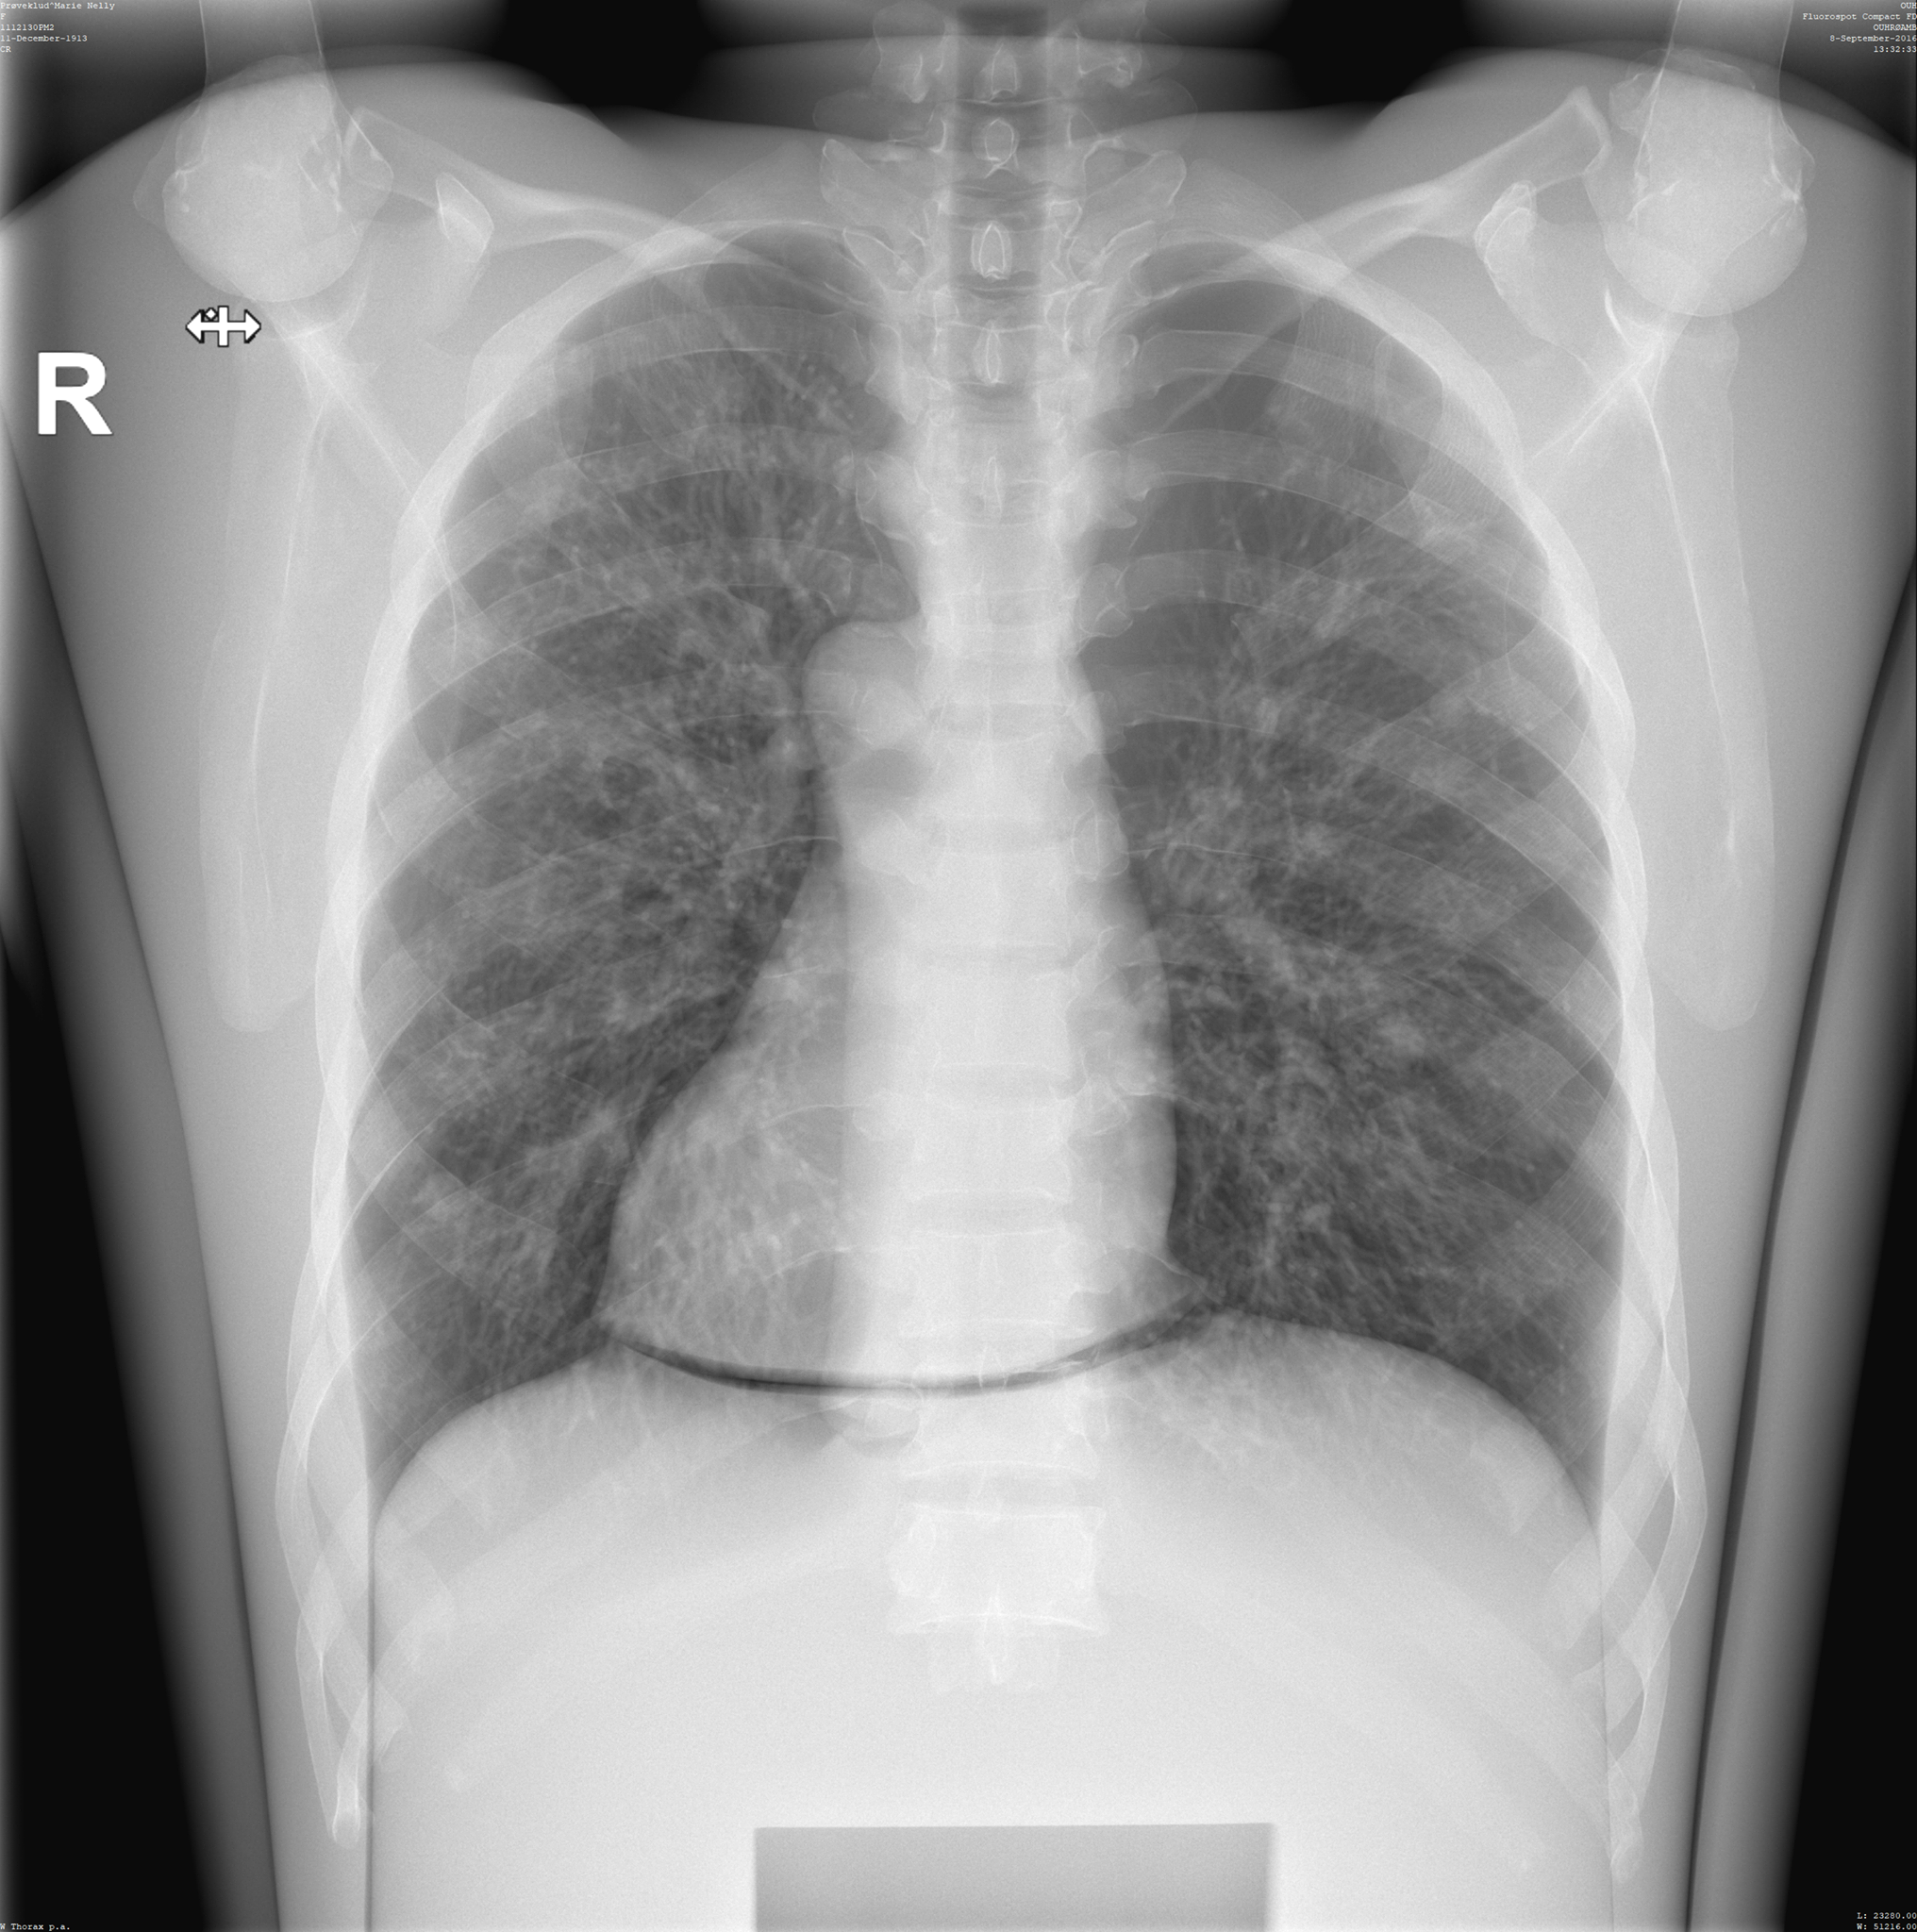
\includegraphics[width=\textwidth]{Image/lung.png} 
    \caption{Billede af lunge.} 
  \end{subfigure} 
  \hfill 
  \begin{subfigure}[b]{0.49\textwidth} 
    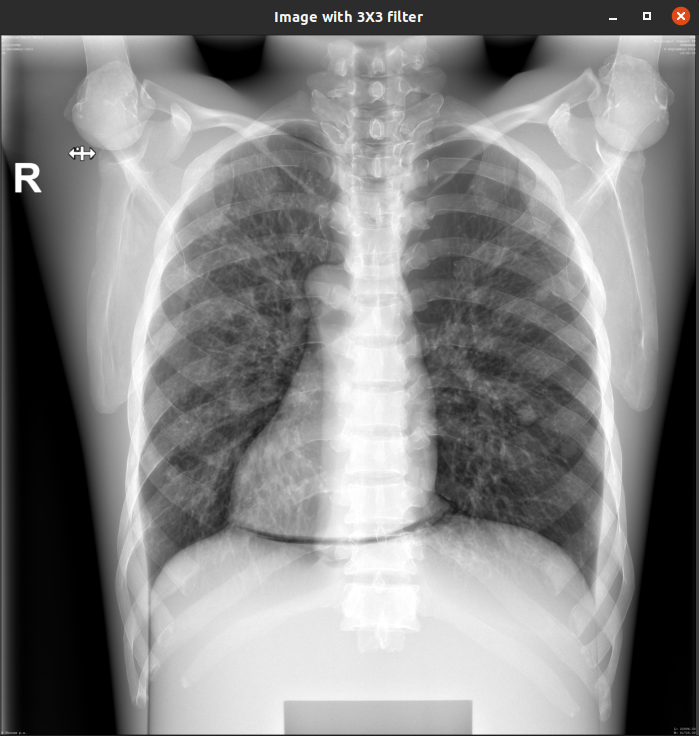
\includegraphics[width=\textwidth]{Image/Image3X3.png} 
    \caption{Filter med 3X3 lunge billede} 
    \label{fig:f5} 
  \end{subfigure} 
    \caption{} 
    \label{fig:image2} 
\end{figure} 

\subsection{Opgave 6} 

På figur \ref{fig:image3} ses på billede (b) et lunge billedet med et 5X5 gausian filter og til højre lungebilledet med et 3X3 gennemsnits filter. Det er svært at se en forskel på de to filter. Gaussian filteret er dog bedre, hvis der skal arbejdes med frekvenser i billedet. 5X5 filteret udtværer kanter i billedet yderligere end et 3X3 filter. 

\begin{figure}[H] 
  \begin{subfigure}[b]{0.49\textwidth} 
    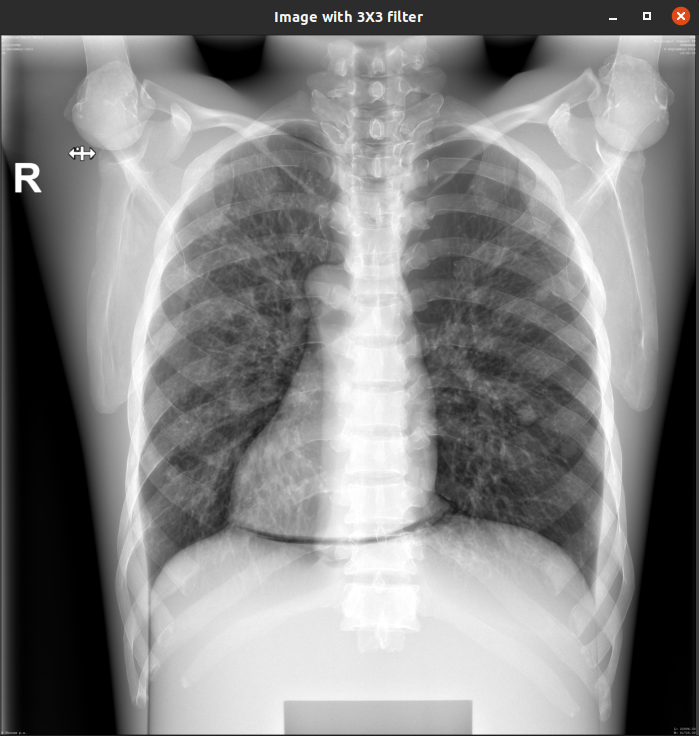
\includegraphics[width=\textwidth]{Image/Image3X3.png} 
    \caption{Filter med 3X3} 
  \end{subfigure} 
  \hfill 
  \begin{subfigure}[b]{0.49\textwidth} 
    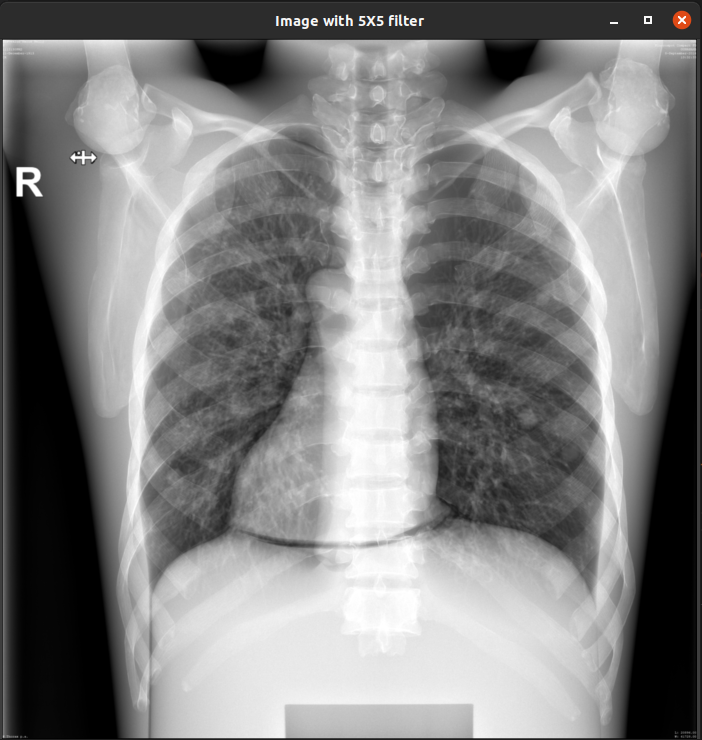
\includegraphics[width=\textwidth]{Image/Image5X5.png} 
    \caption{Filter med 5X5 Gausian} 
    \label{fig:f6} 
  \end{subfigure} 
      \caption{} 
    \label{fig:image3} 
\end{figure} 

  
\subsection{Opgave 7} 

Første skridt i behandlingen af billedet af hjertet var at kigge på billedet af hjertet og histogrammet for at danne et overblik over hvilke værktøjer der ville være godt at bruge og i hvilken rækkefølge.\newline 
Ud fra histogrammet kan det ses at man ikke ville få noget ud af at strække histogrammet. Dette skyldes at der er et meget stort Spike ved 0 og en høj frekvens af 255.\newline Billedet af hjertet viser meget støj. Dette forsøges fjernet ved at bruge et 5X5 Gaussian filter. Dette vil påvirke skrapheden af kanterne men ikke signifikant. 

\begin{figure}[H] 
    \begin{subfigure}[b]{0.49\textwidth} 
        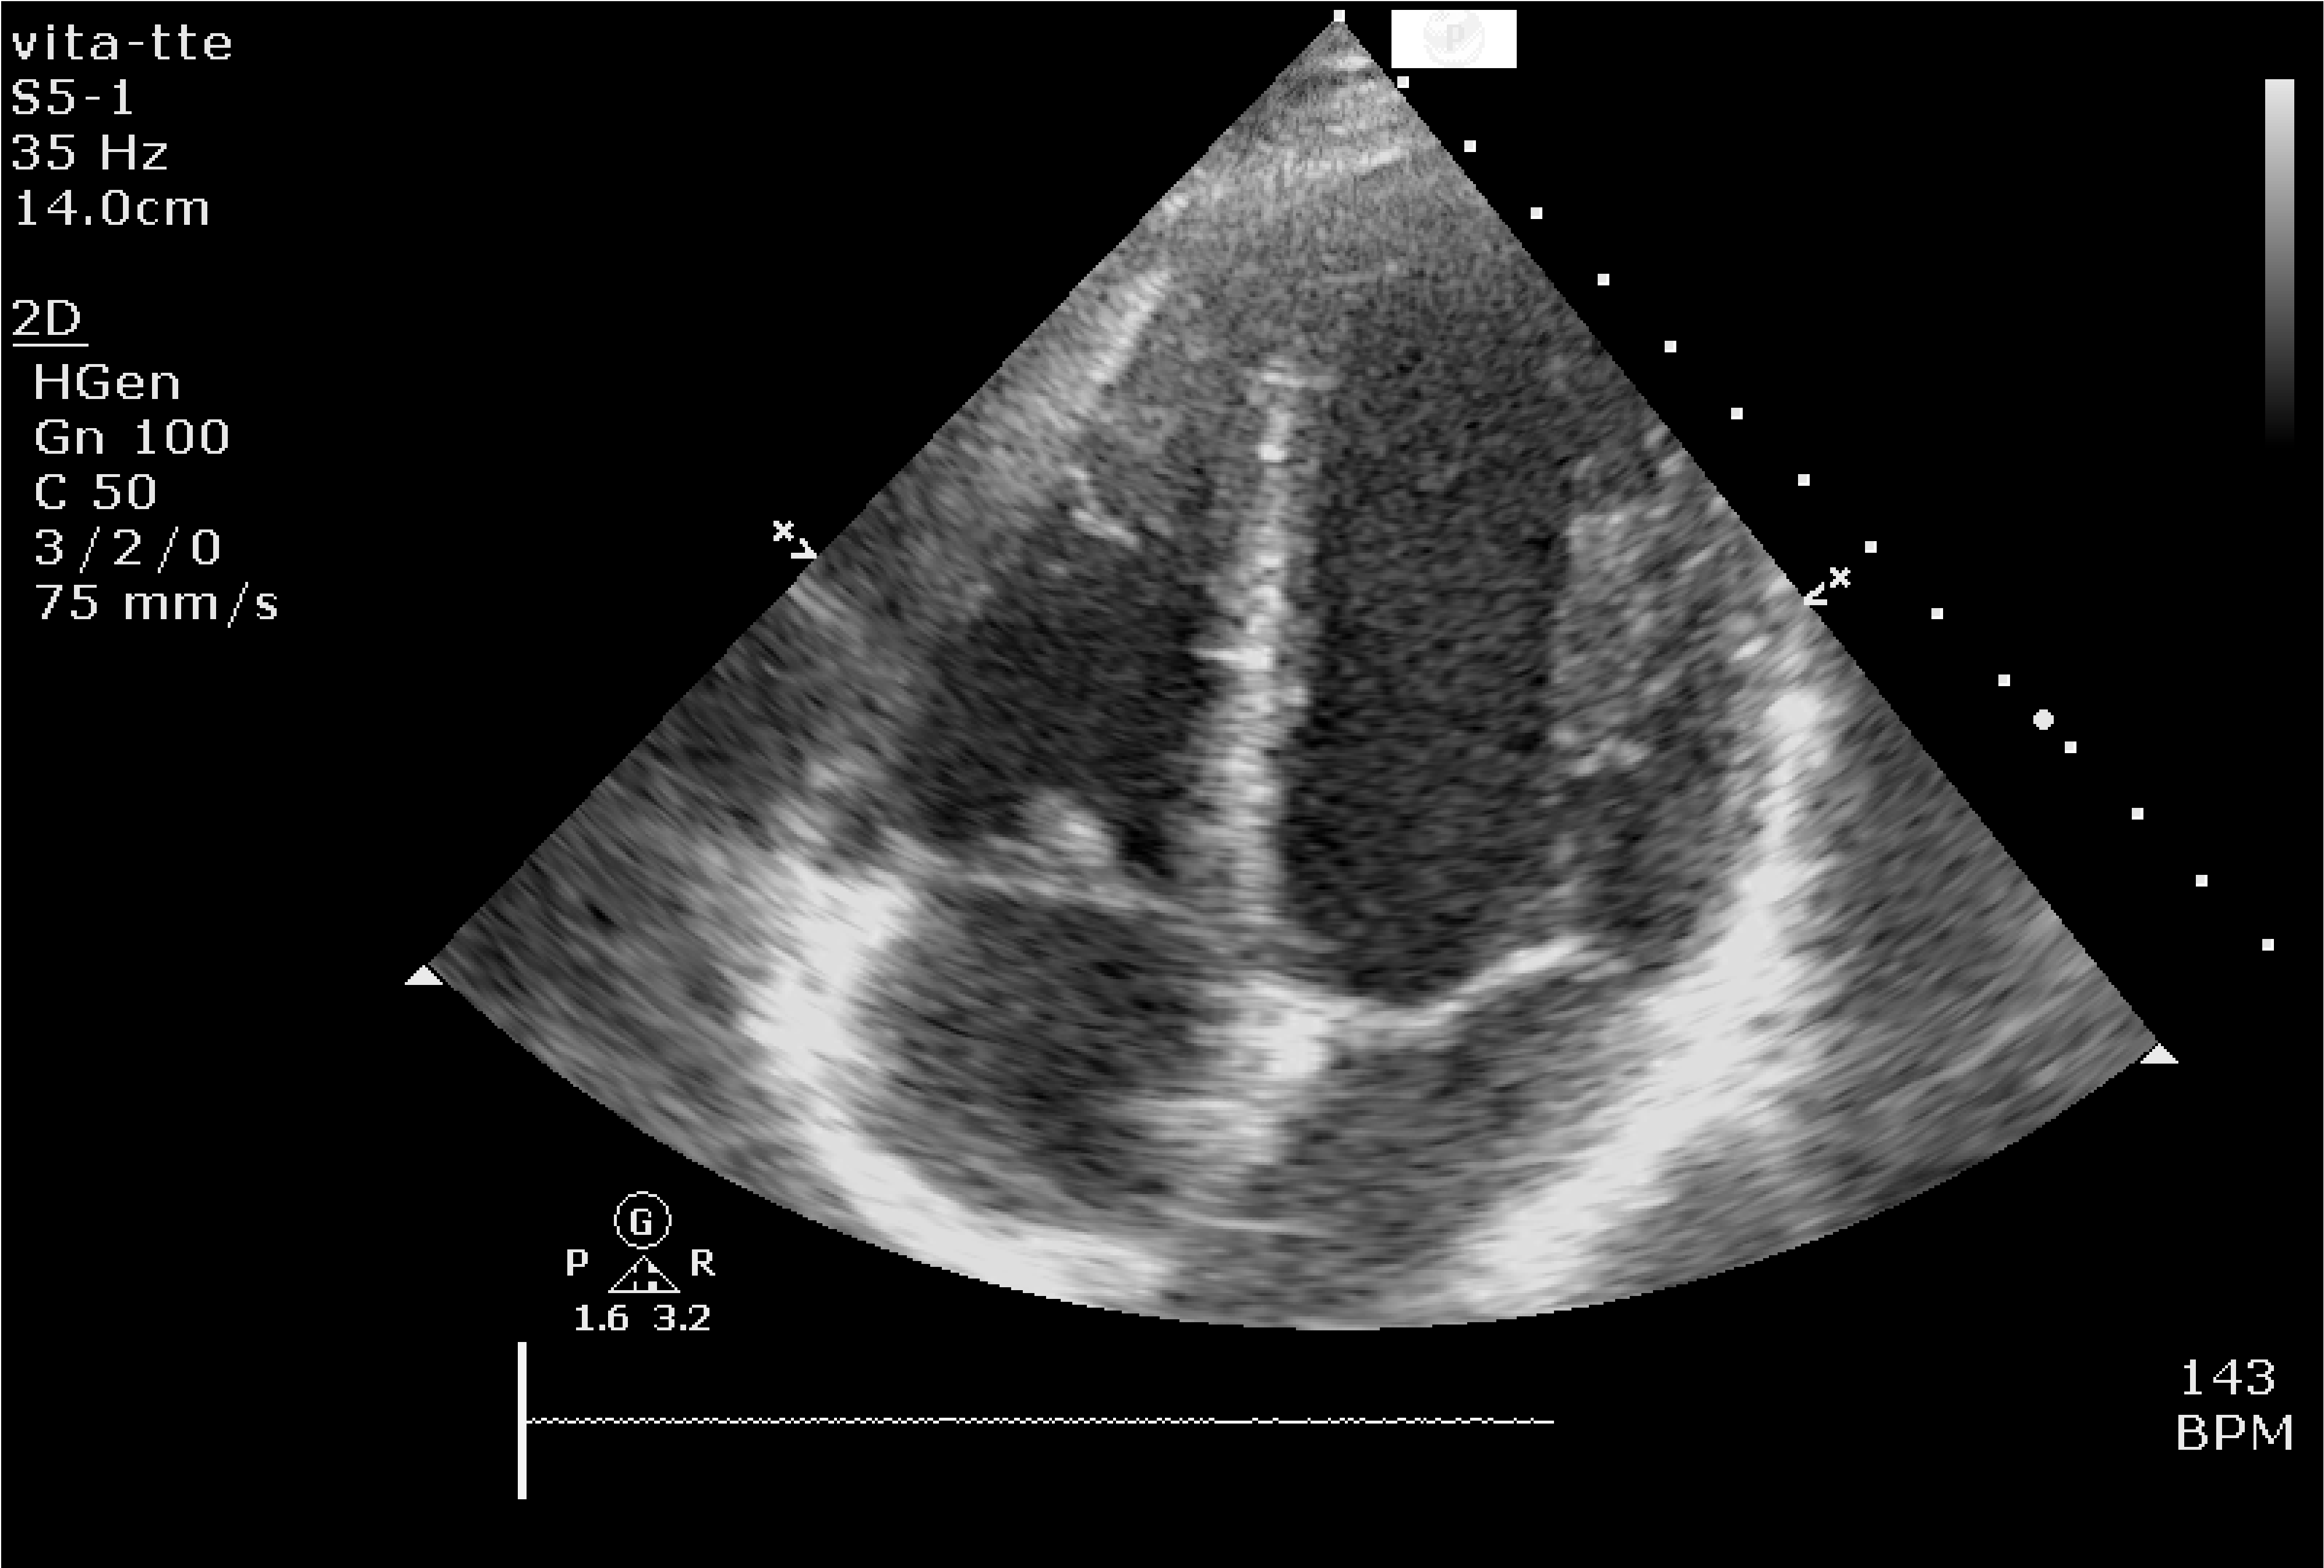
\includegraphics[width=\textwidth]{Image/heart.png} 
        \caption{Original billede af hjerte} 
        \label{fig:f7} 
    \end{subfigure} 
    \hfill 
    \begin{subfigure}[b]{0.49\textwidth} 
        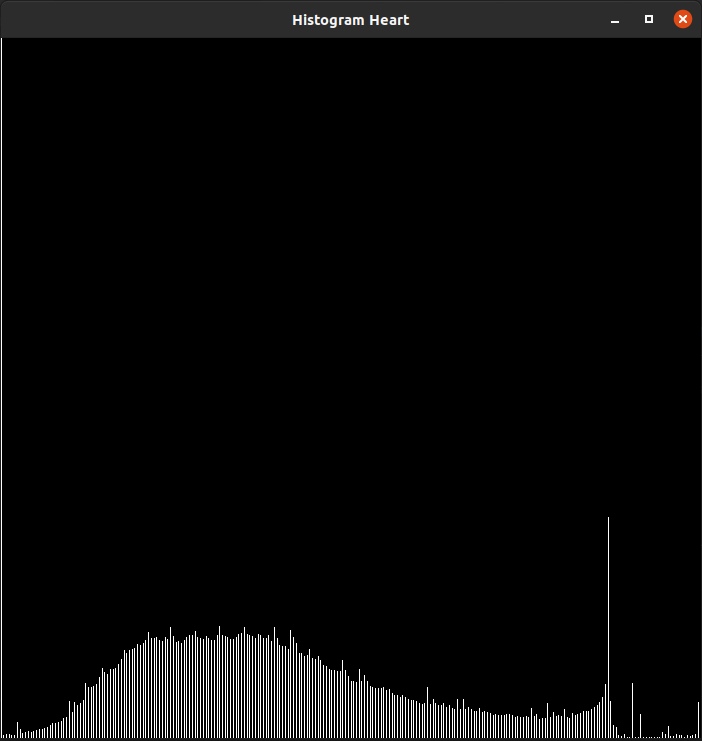
\includegraphics[width=\textwidth]{Image/HistHeart.png} 
        \caption{Histogram af hjerte} 
        \label{fig:f8} 
    \end{subfigure} 
    \caption{} 
    \label{fig:image4} 
\end{figure} 

Næste skridt er at invertere billedet for at fremhæve hjertevægen, som vi gerne vil fremhæve, med sort i stedet for hvid. Dette skidt ændrer ikke billedet. \newline 
Næste skridt er at thredshold billedet i to dele. Billedebehandlingsprogrammet GIMP er blevet brugt til at identificere (Row, Col) værdier i forskellige områder i billedet. Disse er blevet brugt til at thredsholde billedet med forskellige thredshold værdier. Øverste venstre halvdel af billedet er thredsholded med en værdi på 176 og resten af billedet en thredshold værdi på 135. Efterfølgende er det binære billede blevet Eroder og dialated for at optimere på tidligheden af hjertevægen.\newline 
Det færdige resultat ses i \ref{fig:image5} \ref{fig:f10}, hvor hjertevægen og hjerteklapperne er markerede i hvid. 

\begin{figure}[H] 
     \begin{subfigure}[b]{0.49\textwidth} 
        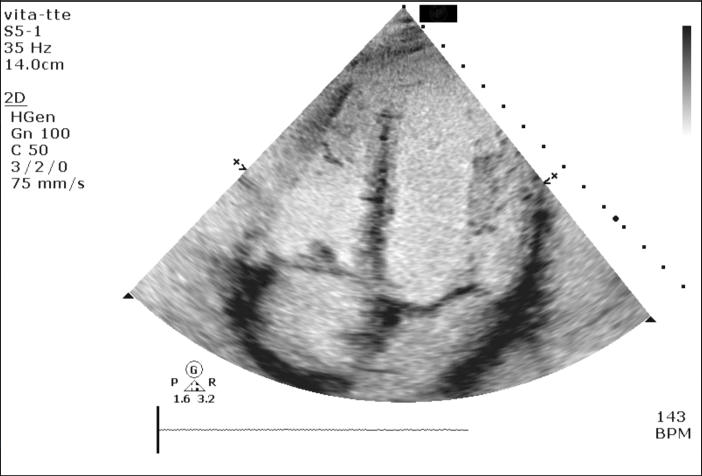
\includegraphics[width=\textwidth]{Image/HeartInvert.png} 
        \caption{Inverted hjerte billede} 
        \label{fig:f9} 
    \end{subfigure} 
     \begin{subfigure}[b]{0.49\textwidth}    
        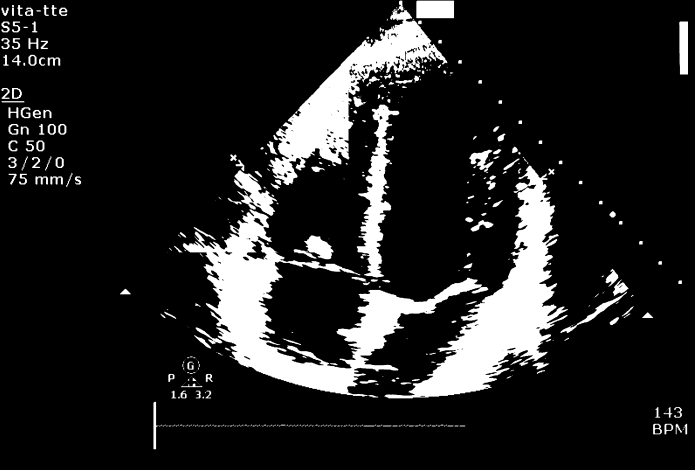
\includegraphics[width=\textwidth]{Image/HeartFinal.png} 
        \caption{Hjerte billede færdig behandlet.} 
        \label{fig:f10} 
    \end{subfigure} 
        \caption{} 
    \label{fig:image5} 
\end{figure} 

  
\newpage 
\section{Decribtion of inverseDFT} 

Funktionen tager som input en string, som er navnet på en fil. Først oprettes objekter: et $Mat <float>$ objekt "IMG" som billedet indlæses til som One channel grayscale. Et Rect objekt der er et rektangel der er samme størrelse som billedet. Et tomt Mat objekt "padded" til at kopiere input billedet over i og tilføjer en ramme af nuller rundt om billedet. \newline 
\begin{lstlisting}[language=c++] 

void inverseDFT(const std::string& filename) { 

     // A gray image 
    cv::Mat_<float> img = cv::imread(filename, cv::IMREAD_GRAYSCALE); 
    cv::Rect origSize(0, 0, img.cols, img.rows); 


    cv::Mat padded; // expand input image to optimal size 
    int m = cv::getOptimalDFTSize(2 * img.rows); 
    int n = cv::getOptimalDFTSize(2 * img.cols);  
    copyMakeBorder(img, padded, 0, m - img.rows, 0, n - img.cols, 
    cv::BORDER_CONSTANT, cv::Scalar::all(0)); 

    cv::Mat_<float> imgs[] = { padded.clone(), 
        cv::Mat_<float>(padded.rows, padded.cols, 0.0f) }; 

\end{lstlisting} 
Der oprettes herefter et Mat objekt med to channels $"img dft"$ hvor "img" meres over i. Dette gøres ved et 1-channel billedede for at gøre det muligt at arbejde med komplekse tal. \newline 
dtf funktionen laver en Discrete Fourier transform og overskriver imgdft med de nye værdier. \newline 
Efter DFT spilttes over i imgs 2-channels. Så den relle del af DFT ligger i imgs[0] og den imaginære del i imgs[1]. \newline 
Der oprettes to elementer, magnitude og phase. Efterfølgende ændres imgs[0] og imgs[1] fra cartesian koordinater til polare som gemmes i hhv. magnitude og phase. \newline 
dtfshift funktionen flytter rundt på kvadranterne så top-venstre og bund-højre bytter plads og top-højre og bund-venstre bytter plads. \newline 
Herefter tages logaritmen af magitude + 1 og imgout oprettes. \newline 

\begin{lstlisting}[language=c++] 
    // Merge 
    cv::Mat_<cv::Vec2f> img_dft; 
    cv::merge(imgs, 2, img_dft); 

    // Compute DFT 
    cv::dft(img_dft, img_dft); 

    // Split 
    cv::split(img_dft, imgs); 

    // Compute magnitude/phase 
    cv::Mat_<float> magnitude, phase; 
    cv::cartToPolar(imgs[0], imgs[1], magnitude, phase); 

    // Shift quadrants for viewability 
    dftshift(magnitude); 

    cv::Mat_<float> orig_magnitudel = magnitude + 1.0f; 
    cv::log(orig_magnitudel, orig_magnitudel); 

    // Output image 
    cv::Mat_<float> imgout; 
\end{lstlisting} 


ILP finder halvdelen af den mindste længde af billedet og definere en cutoff frekvens. fs sættes til halvdelen af den mindste side (rows, cols) og ganges med cutoff frekvensen. \newline 
Herefter oprettes et mat objekt "filter" bestående af nuller med et rektangel med origo i midten af filter. Rektanglet har højden og bredden fs*2. \newline 

\begin{lstlisting}[language=c++] 

    // // ILP 
    float halfOfSmallestImageSide = std::min(img_dft.rows, img_dft.cols) / 2.0; 
    float D0 = 0.3;  
    int fS = halfOfSmallestImageSide * D0; 
    cv::Mat filter(img_dft.rows, img_dft.cols, img_dft.type(), 
        cv::Scalar(0.0, 0.0)); 
    filter(cv::Rect(filter.cols / 2 - fS, filter.rows / 2 - fS, fS * 2.0, fS * 2.0)) = 
        cv::Scalar(1.0, 0.0); 
\end{lstlisting} 

 I næste frekvens splittes filter som tidligere til imgs to kanaler. Der laves en omregning fra cartesian koordinater til polare og de gemmes i magnitude og phase. dtfshift funktionen flytter rundt på kvadranterne og mulSpectrums tager imgdft, plusser den med filter og gemmer den i imgdft.\newline 
Herefter splittes imgdft igen ind i imgs. Der sker igen en omregning fra cartesian koordinater til polare og de gemmes i magnitude og phase. \newline 
Der oprettes et Mat<float> objekt final magnitudel som får værdien magnitude + 1. Herefter bytter dftshift om på kvadranterne og final magnitudel laves om til log skala. \newline 

\begin{lstlisting}[language=c++] 
    cv::split(filter, imgs); 
    cv::cartToPolar(imgs[0], imgs[1], magnitude, phase); 
    cv::imshow("Filter", magnitude); 

    dftshift(filter); 

    cv::mulSpectrums(img_dft, filter, img_dft, 0); 
    cv::split(img_dft, imgs); 
    cv::cartToPolar(imgs[0], imgs[1], magnitude, phase); 

    cv::Mat_<float> final_magnitudel; 
    final_magnitudel = magnitude + 1.0f; 
    
    dftshift(final_magnitudel); 
    cv::log(final_magnitudel, final_magnitudel); 
\end{lstlisting} 

Den sidste del af koden udregner den inverse DFT med dft funktion. dft funktion kan regne begge vej. imgdft er input og imgout er output. Funktionen omregner fra frekvensdomænet tilbage til pixels og skalere derefter resultatet. \newline 
Herefter normaliseres img, orig magnitudel, final magnitudel og phase mellem 0 og 1 og billederne vises. \newline 
imgout ændres til samme størrelse som orig, normaliseres mellem 0 - 1 og vises. orig magnitudel normaliseres mellem 0 - 255 og gemmes som png.\newline 

\begin{lstlisting}[language=c++] 

    // Do inverse DFT 
    cv::dft(img_dft, imgout, 
    cv::DFT_INVERSE + cv::DFT_SCALE + cv::DFT_REAL_OUTPUT); 

    // Show 
    cv::normalize(img, img, 0.0, 1.0, cv::NORM_MINMAX); 
    cv::normalize(orig_magnitudel, orig_magnitudel, 0.0, 1.0, cv::NORM_MINMAX); 
    cv::normalize(final_magnitudel, final_magnitudel, 0.0, 1.0, cv::NORM_MINMAX); 
    cv::normalize(phase, phase, 0.0, 1.0, cv::NORM_MINMAX); 
    cv::imshow("Input", img); 
    cv::imshow("Original magnitude", orig_magnitudel); 
    cv::imshow("New magnitude", final_magnitudel); 

    imgout = imgout(origSize); 
    cv::normalize(imgout, imgout, 0.0, 1.0, cv::NORM_MINMAX); 
    cv::imshow("Output", imgout); 
    cv::waitKey(); 
    cv::normalize(orig_magnitudel, orig_magnitudel, 0.0, 255.0, cv::NORM_MINMAX); 
    cv::imwrite("orig_magnitude.png", orig_magnitudel); 
\end{lstlisting} 

Opsummeret tager funktionen et billede: 

\begin{itemize} 
    \item Forbereder det til en Discrete Fourier transform  
    \item Laver transformationen 
    \item Laver et filter som transformeres og ligges til billedets magnitude og phase.  
    \item Magnitude plusses med 1 og omregnes til log.  
    \item Billedet invers transformeres.  
    \item Billede magnituderne og phasen normaliseres mellem 0 -1  og vises 
    \item Output normaliseres mellem 0 -1 og vises   
    \item Orig gemmes efter den er blevet normaliserede mellem 0 - 255 . 
\end{itemize} 
\end{document} 

 